\chapter{Testing e Benchmarking}

Ai fini di verificare il corretto funzionamento del sistema e valutarne le prestazioni, sono stati sviluppati una serie di test e benchmark. Firegex già presentava un set di test, che con l'integrazione di nfproxy sono stati ampliati e migliorati, al fine di coprire anche le nuove
feature introdotte.\\
I test sono eseguiti prima di ogni rilascio in automatico, al fine di garantire che le modifiche apportate non abbiano introdotto regressioni. I rilasci di firegex avvengono tramite GitHub Actions, che ad ogni rilascio su GitHub esegue i test e, in caso di successo, pubblica l'immagine del container sul Github Container Registry (ghcr.io/pwnzer0tt1/firegex) e rilascia una nuova versione della libreria, inclusa nello stesso repository, su PyPi.\\
I rilasci avvengono sia per architetture \texttt{x86\_64} che \texttt{ARM64}, al fine di supportare il maggior numero di macchine possibile.

\section{Integrazione dei test}

Tutti i test di firegex sono disponibili nel suo repository, all'interno della cartella \texttt{tests}.\\
In particolare, quelli riguardanti nfproxy sono contenuti nel file \texttt{tests/nfproxy\_test.py}, ed esegue la seguente serie di operazioni:

\begin{itemize}
    \setlength{\itemsep}{1pt}
    \setlength{\parskip}{1pt}
    \item Avvia un nuovo servizio sull'interfaccia di loopback, e verifica che il traffico non sia stato compromesso dal semplice avvio del modulo.
    \item Verifica che ogni tipo di statment sia correttamente funzionante, inserendo un filtro che individua se sul segmento TCP sia presente un payload specifico, che se inviato, causi il comportamento desiderato, imposto dallo statment inserito.
    \item Si verifica che la funzionalità di modifica funzioni correttamente, eseguendo prove sia su mangle a pacchetti più piccoli, che a pacchetti più grandi, comprovando pertanto che la traduzione degli ack e seq avvenga correttamente. Inoltre viene verificato se a seguito della modifica, il traffico di rete continui a transitare normalmente.
    \item Si assiucura che le funzionalità di interruzione del servizio e del singolo pyfilter sia correttamente funzionante.
    \item Per ogni tipo di datahandler, si scambiano dei payload di prova al fine di verificare se il parsing dei vari dati avvenga correttamente. Datahandler testati: \texttt{TCPInputStream}, \texttt{TCPOutputStream}, \texttt{HttpRequest}, \texttt{HttpResponse}, \texttt{HttpRequestHeader},
    \texttt{HttpResponseHeader} includendo anche il parsing di \texttt{Frame websocket}.
    \item Vengono testate tutte le API backend di nfproxy, verificando che le chiamate restituiscano i valori corretti, e si comportino in modo coerente alla loro funzione.
    \item Si verifica inoltre che vengano conteggiate correttamente le connessioni bloccate, e i pacchetti modificati nelle statistiche.
\end{itemize}

\section{Benchmark}

I benchmark sono stati realizzati tramite uno script python con l'ausilio di \texttt{iperf3}\footcite{\url{https://iperf.fr/}}{iperf_website}.\\
Le casistiche utilizzate sono di semplice natura: verificano le prestazioni in termini di throughput, e lo fanno sia a servizio attivo senza filtri, che con un filtro che applica la seguente regex al payload TCP (regex per il matching di email):
\begin{verbatim}
(?:[a-z0-9!#$%&'*+/=?^_`{|}~-]+
    (?:\.[a-z0-9!#$%&'*+/=?^_`{|}~-]+)* |
    "(?:[\x01-\x08\x0b\x0c\x0e-\x1f\x21\x23-\x5b\x5d-\x7f] |
        \\[\x01-\x09\x0b\x0c\x0e-\x7f])*")
@
(?:(?:[a-z0-9](?:[a-z0-9-]*[a-z0-9])?\.)+
    [a-z0-9](?:[a-z0-9-]*[a-z0-9])? |
    \[(?:(?:25[0-5] | 2[0-4][0-9] | [01]?[0-9][0-9]?)\.){3}
        (?:25[0-5] | 2[0-4][0-9] | [01]?[0-9][0-9]? |
            [a-z0-9-]*[a-z0-9]:
            (?:[\x01-\x08\x0b\x0c\x0e-\x1f\x21-\x5a\x53-\x7f] |
                \\[\x01-\x09\x0b\x0c\x0e-\x7f])+)\])
\end{verbatim}

A differenza dei test, i benchmark non hanno lo scopo di applicare i filtri su un traffico da bloccare, ma si inserisce la seguente regola all'unico scopo di
misurare l'overhead causato dalla presenza del filtro stesso.\\
I benchmark sono stati eseguiti su una macchina con le seguenti caratteristiche:
\begin{listing}[H]
    \begin{minted}[
        frame=single,
        framerule=0.8pt,
        fontsize=\footnotesize,
        breaklines
      ]{text}
Macbook Air M2 16GB RAM
Su una VM avviata da OrbStack con Fedora Linux 41 (Container Image) aarch64
Linux 6.12.13-orbstack-00304-gede1cf3337c4
\end{minted}
\end{listing}

Lo script python che esegue i benchmark, ripete la stessa misura un numero configurabile di volte, sia per il modulo nfproxy, che per il modulo nfregex.
I risultati sono stati raccolti e analizzati, e messi a disposizioni nei grafici in seguito, eseguiti con i seguenti comandi:
\begin{listing}[H]
    \begin{minted}[
        frame=single,
        framerule=0.8pt,
        fontsize=\footnotesize,
        breaklines
      ]{bash}
python3 comparemark.py nfproxy -p testpassword -d 1 -s 50 -V 100
python3 comparemark.py nfregex -p testpassword -d 1 -s 50 -V 100
\end{minted}
\end{listing}

I benchmark pertanto sono stati eseguiti con 1 secondo di durata della singola misura, 50 connessioni simultanee, e 100 misure eseguite. Il numero indicato dopo la \texttt{T} nei grafici indica il numero di thread con cui firegex è stato configurato: quindi eseguiti sia in single-threading che in multi-threading (con 8 thread).

\begin{figure}[H]
    \centering
    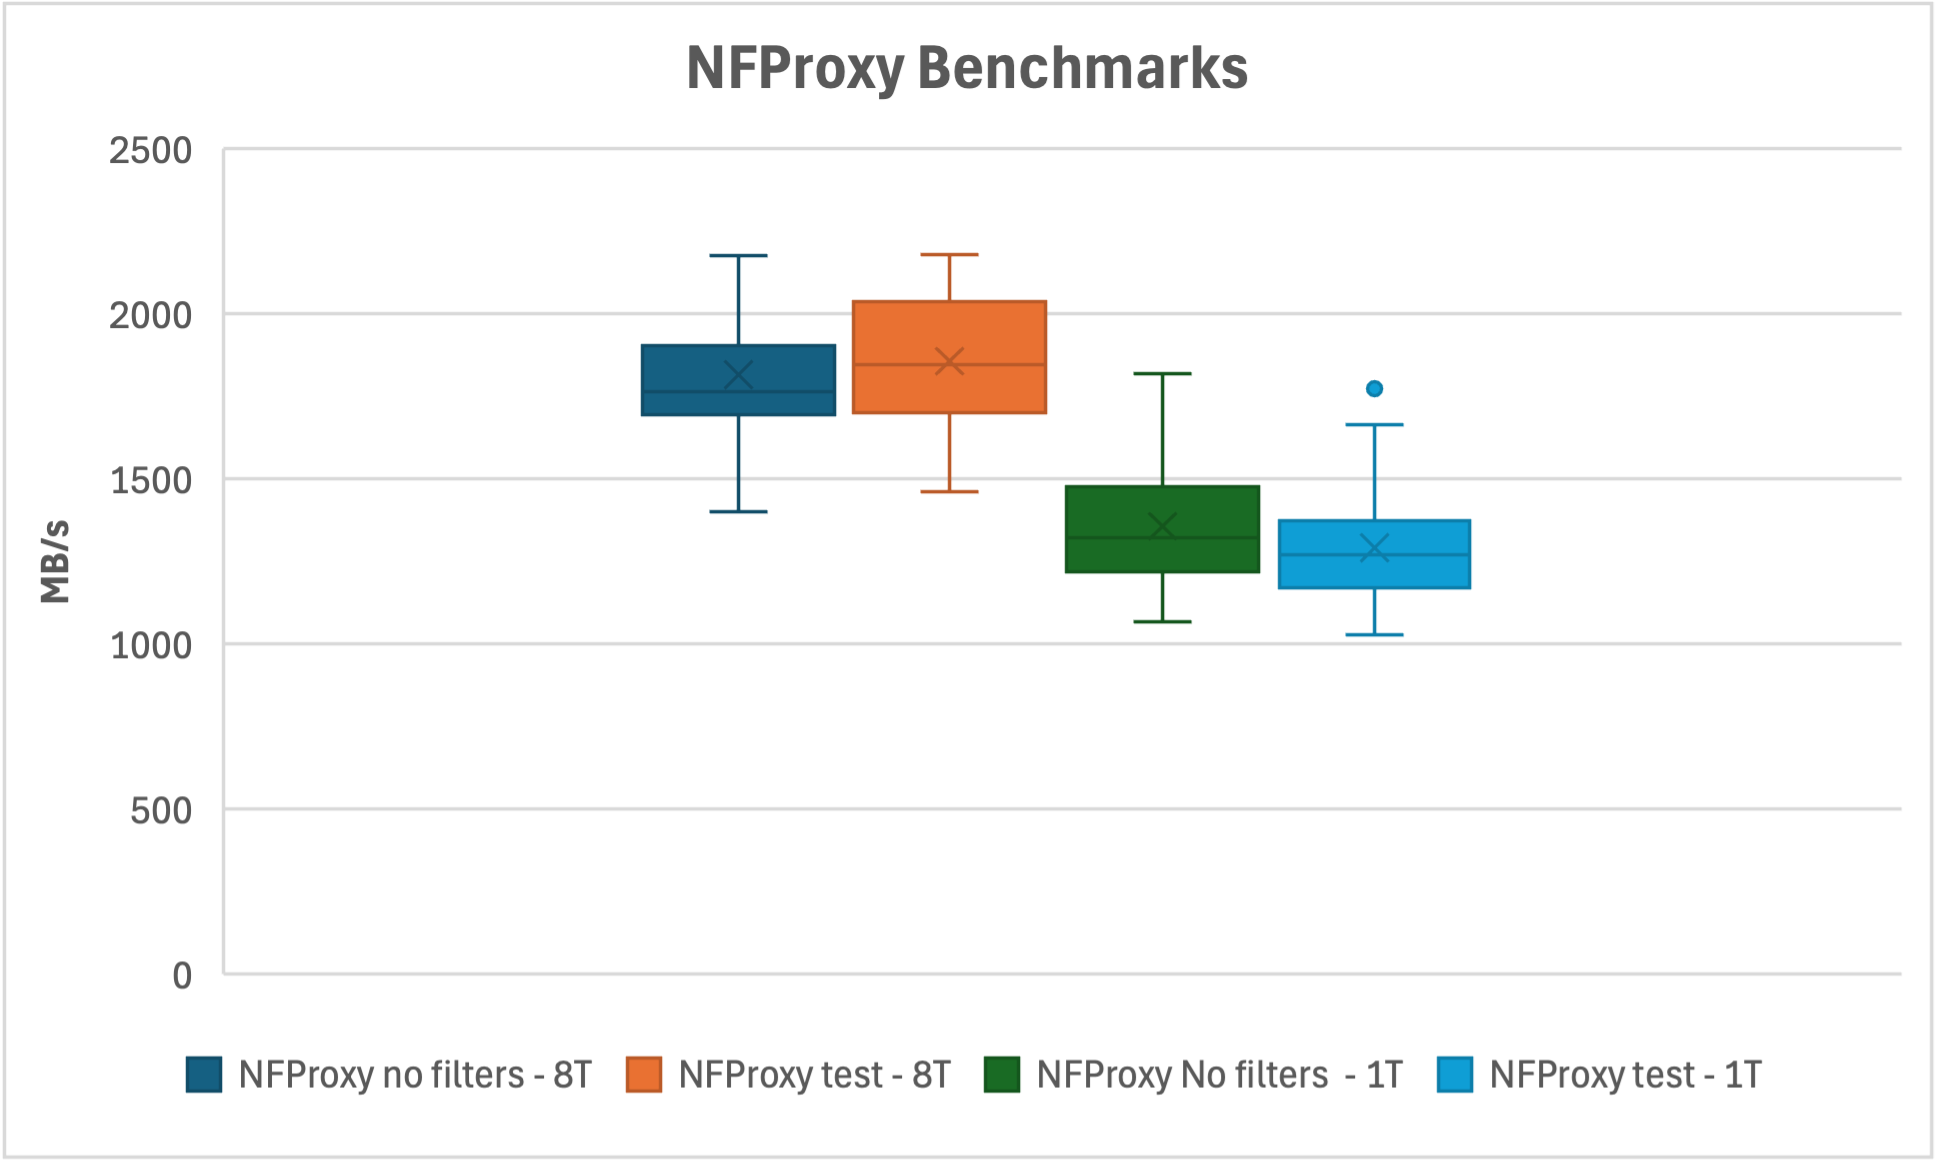
\includegraphics[width=0.90\textwidth]{images/chapter4/whisker_nfproxy.png}
    \caption{Grafico Whisker sulle misure di throughput di nfproxy}\label{fig:wisker_nfproxy}
\end{figure}

Si può notare come le performance in multi-threading di nfproxy siano migliori rispetto all'utilizzo del singolo thread. È importante sottolineare come nei benchmark non viene eseguito alcun tipo di elaborazione riguardo il parsing dei dati, pertanto il carico di elaborazione è comunque limitato.\\

\begin{figure}[H]
    \centering
    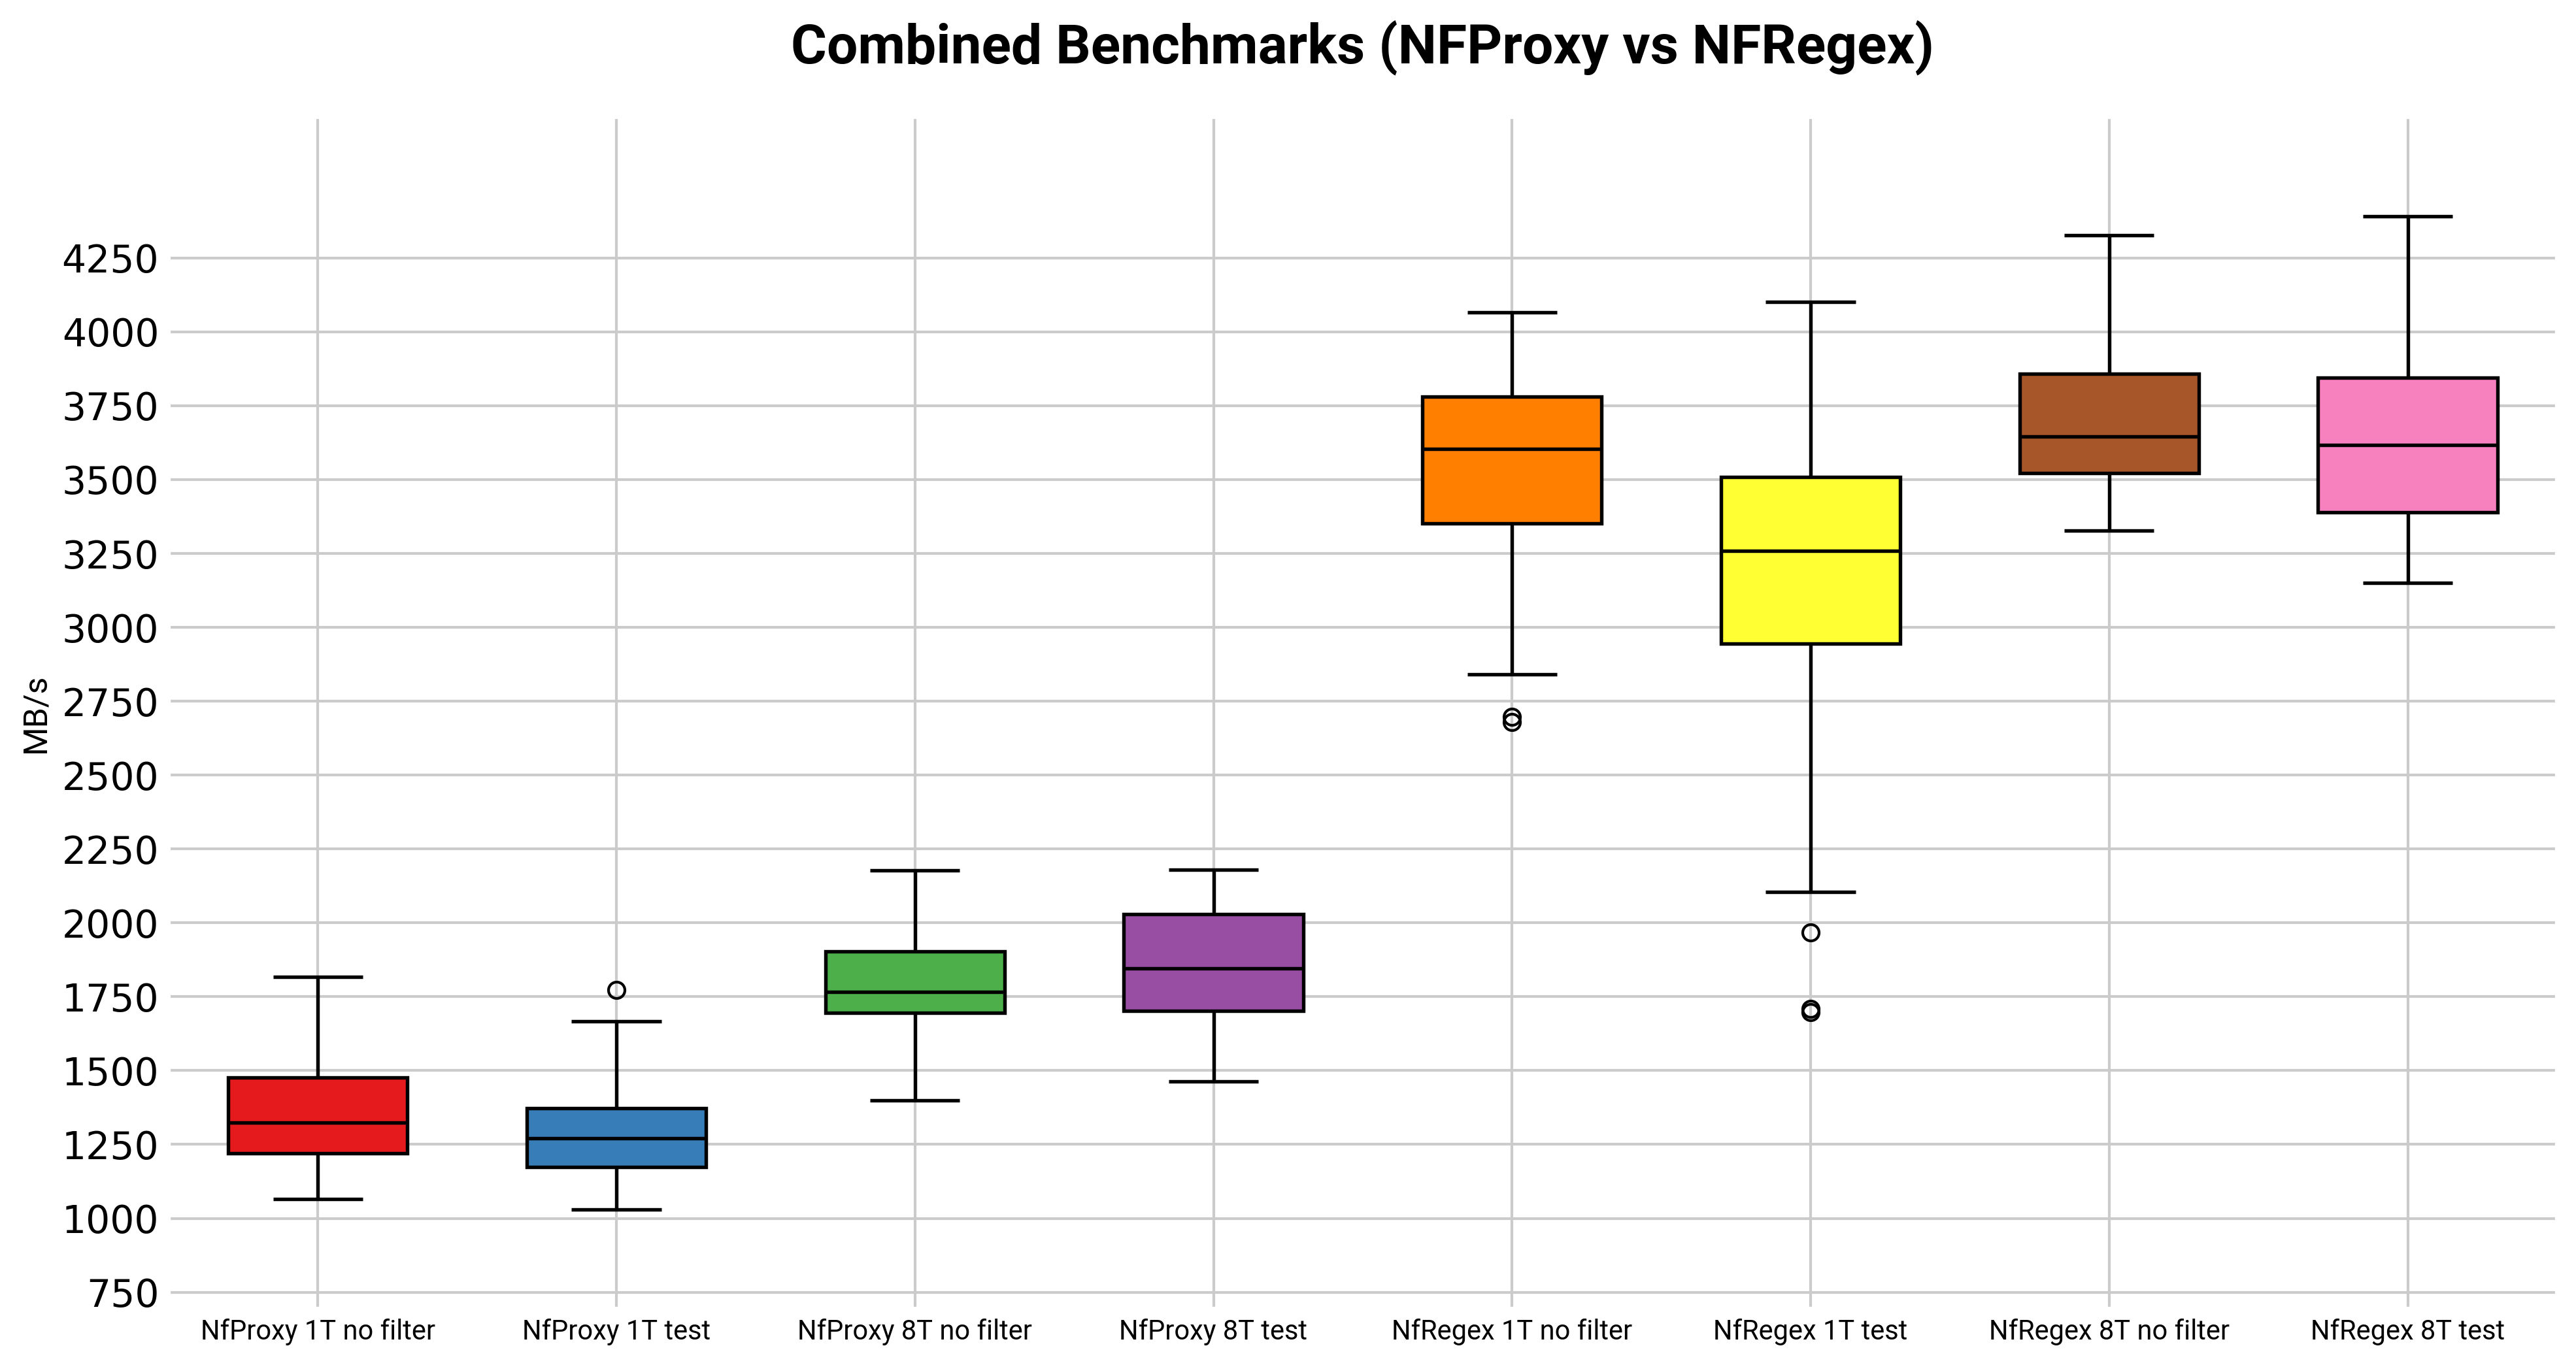
\includegraphics[width=0.98\textwidth]{images/chapter4/whisker_compare.png}
    \caption{Grafico Whisker sulle misure di throughput di nfproxy e nfregex}\label{fig:wisker_nfproxy_nfregex}
\end{figure}

Dal confronto di nfproxy e nfregex si può notare come nfproxy abbia un calo di prestazioni rilevante rispetto a nfregex, che tuttavia rimane comunque abbondantemente alto per supportare anche carichi di rete molto elevati.\\
